\documentclass[oneside]{book}

\usepackage[utf8]{inputenc}
\usepackage[english]{babel}

\usepackage{titlesec}
\usepackage{fancyhdr}
\usepackage{graphicx}
\usepackage{caption}

\usepackage[a4paper, total={6in, 8in}]{geometry}
\usepackage{setspace}

\usepackage{amssymb}
\usepackage{amsmath}

\usepackage{cancel}
\usepackage{array}
\usepackage{environ}
\usepackage{textcomp}

\usepackage{hyperref}

\title{Binary Subtraction and the Half-Subtractor}
\author{Liam Gardner}
\date{\today}

\graphicspath{ {figs/} }

\hypersetup{
    colorlinks,
    citecolor=black,
    filecolor=black,
    linkcolor=blue,
    urlcolor=black
}

\titleformat
{\chapter} % command
[display] % shape
{\bfseries\Large\itshape} % format
%{Story No. \ \thechapter} % label
{}
{0ex} % sep
{
    \rule{\textwidth}{1pt}
    \vspace{1ex}
    \centering
} % before-code
[
\vspace{-1.8ex}%
\rule{\textwidth}{1pt}
] % after-code

\renewcommand{\chaptermark}[1]{%
\markboth{#1}{}}
\newcommand{\Mod}[1]{\ (\mathrm{mod}\ #1)}

\pagestyle{fancy}
\fancyhf{}
\fancyhead[LE,RO]{Binary Subtraction and the Half-Subtractor}
\fancyhead[RE,LO]{\thechapter: Interviewing Subtraction}
%\fancyfoot[CE,CO]{\leftmark}
%\fancyfoot[LE,RO]{\thepage}
\cfoot{\thepage}

\onehalfspace

\begin{document}

\newcommand\tab[1][1cm]{\hspace*{#1}}

\maketitle
\tableofcontents
\chapter{An interview with subtraction}
\markboth{An interview with subtraction}{}
\tab
Subtraction is taught at a very basic level. Here in Canada, it's taught roughly in grade one or two. One of the things that always confused me was the concept of borrowing. Looking back on it, I'm less so confused, but more so disturbed by the way it was taught. As an example, let's go through the following subtraction statement.
\begin{center}
\begin{tabular}{c c c c c}
& 1 & 2 & 2 & 4 \\
- & & 6 & 4 & 3 \\
\end{tabular}
\end{center}
\tab
The algorithm works by starting from the rightmost digit, which in this instance is $4-3$, and perform the basic subtraction under the circumstance that the minuend (the first number) is greater than the subtrahend (the second number). In this case, we can see that this is true, and perform the subtraction to attain a value of 1.
\begin{center}
\begin{tabular}{c c c c c}
& 1 & 2 & 2 & 4 \\
- & & 6 & 4 & 3 \\
\hline
& & & & 1 \\
\end{tabular}
\end{center}
\tab
Moving to our next value, we can see that $2-4$ does not meet the requirement. As a standalone operation, $2-4=-2$. However, this is not standalone, and is instead based around a bigger ``problem''. In school, we are taught to perform something called \textit{borrowing}. This is when you usurp a value from the successive digit and add 10 to the digit we're working with. In our case, the successive digit is $2$. The algorithm tells us to subtract $1$ from the successive value, and add $10$ to the current value we're working with. This is the concept of borrowing. Now, we can proceed with the basic subtraction. $12-4 = 8$. Therefore, the next digit in our difference is $8$.
\begin{center}
\begin{tabular}{c c c c c}
& 1 & \xcancel{2}1 & 12 & 4 \\
- & & 6 & 4 & 3 \\
\hline
& & & 8 & 1 \\
\end{tabular}
\end{center}
\tab
When I first learned this, it wasn't just unintuitive to me, I was completely incapable of understanding what was happening. This algorithm for subtraction requires the performer to understand how to subtract two numbers normally. For a computer, this is completely fine, however as a method for teaching children, it was a nightmare. Furthermore, most elementary teachers can't go into too much detail as to how this algorithm works, it was ingrained into their brain and they were told to ingrain it into ours. For now, I'll complete the table with each step before continuing.
\begin{center}
\begin{tabular}{c c c c c}
& \xcancel{1}0 & 11 & 12 & 4 \\
- & & 6 & 4 & 3 \\
\hline
& & 5 & 8 & 1 \\
\end{tabular}
\end{center}
\begin{center}
\begin{tabular}{c c c c c}
& 1 & 2 & 2 & 4 \\
- & & 6 & 4 & 3 \\
\hline
& & 5 & 8 & 1 \\
\end{tabular}
\end{center}
\chapter{Subtraction via modular arithmetic}
\markboth{Subtraction via modular arithmetic}{}
\fancyhead[RE,LO]{\thechapter: Decimal subtraction via modular arithmetic}
\tab
\textbf{I would like to start this section by saying that this has no immediately visible applications as to what we have been taught, but instead exists only to provide insight as to the concept of subtraction's borrowing.} To begin, let's take a look at modular arithmetic in base 10. The modulo operator works by taking the remainder of the division by 10. That is, for any function $f(x)$, $f(x)\mathrm{\,\,mod\,\,} 10$ is the same as saying  ``divide $f(x)$ by 10, and return the remainder.'' For some basic pretense, $\forall x \in [0,10), x\mathrm{\,\,mod\,\,}10 = x$. Here are some more values in what is known as $\mathbb{Z}_10$.

\begin{center}
\begin{tabular}{|c|c|c|c|c|c|}
\hline
x values & -5 & -4 & -3 & -2 & -1 \\
\hline
$x$ mod 10 & 5 & 6 & 7 & 8 & 9\\
\hline
x values & 11 & 12 & 13 & 14 & 15\\
\hline
$x$ mod 10 & 1 & 2 & 3 & 4 & 5\\
\hline
x values & -30 & -29 & -28 & -27 & -26 \\
\hline
$x$ mod 10 & 0 & 1 & 2 & 3 & 4 \\
\hline 
\end{tabular}
\end{center}
\tab
All numbers will wrap around to end up on the interval $[0,10)$. Calculations that end with the result mod 10 can be said to be part of a set called $\mathbb{Z}_{10}$. This is because all all output values will end up in the interval $[0,10)$. Typically, operations in integer rings such as $\mathbb{Z}_{10}$ will only have inputs in that interval as well. Since digit subtraction will always have the minuend and subtrahend be within that interval, it wouldn't be incorrect to say that they take place in the integer ring $\mathbb{Z}_{10}$. In later sections, we will be moving into the binary system, which means operations will exist in the integer ring $\mathbb{Z}_2$ rather than $\mathbb{Z}_{10}$, and all values will exist on the interval $[0,2)$. 
\newline
\tab
A different subtraction algorithm can be created as follows:
\begin{itemize}
	\item Align subtraction vertically, in the same way as the conventional algorithm.
	\item We read from right to left. Start with the two rightmost digits.
	\item Perform the single-digit subtraction.
	\item Take the calculated difference, mod 10 and write that digit below your aligned numbers.
	\item If the minuend was less than the subtrahend, place an indicator above the successive digits.
	\item Repeat process for all remaining digits.
	\item For all digits with an indicator above them, subtract 1 from the final digit.
	\item The remaining value is your difference. All numbers with indicators above them had been borrowed from.
\end{itemize}
\tab
For the time being, we'll call this algorithm \textit{modular subtraction}. This new algorithm fixes two problems: the first is that it removes the problem I had with having two-digit numbers in places meant to hold one digit (which probably shouldn't be considered an objective problem). The second is a problem that I haven't spoken of yet. Using the normal subtraction algorithm, subtracting numbers $2n-n,\, n \in \mathbb{N} \mid \{5\leq n < 10\}$ will end up with repetition. As an example, let's take a look at subtracting $10-5$ and $18-9$.
\begin{center}
\setlength{\tabcolsep}{1pt}
\begin{tabular}{c c c}
 & 1 & 0 \\
- & & 5\\
\end{tabular}
\end{center}
\tab
As per the normal subtraction algorithm, since $0 < 5$, we borrow from the successive digit. This process will result in the following
\begin{center}
\setlength{\tabcolsep}{2.5pt}
\begin{tabular}{c c c}
&\xcancel{1}0 & 10 \\
-&&5 \\
\end{tabular}
\end{center}
\tab
We end up in this loop, having to repeat this process infinitely. As a result, most children will learn to memorize the answers to certain problems like this. As another example, here's what happens with $18-9$.
\begin{center}
\setlength{\tabcolsep}{1pt}
\begin{tabular}{c c c}
&1&8\\
-&&9\\
\end{tabular}
\end{center}
\begin{center}
\setlength{\tabcolsep}{2.5pt}
\begin{tabular}{c c c}
 &\xcancel{1}0 & 18\\
-& & 9\\
\end{tabular}
\end{center}
\tab
We'll get to solving this problem with modular subtraction later. For now, let's take a look at our original problem. The first step is to re-create the same setup we'd use conventionally.
\begin{center}
\begin{tabular}{c c c c c}
& 1 & 2 & 2 & 4 \\
- & & 6 & 4 & 3
\end{tabular}
\end{center}
\tab
Next, we look at and subtract the rightmost two digits. $4-3=1$. Now, we take the remainder of that difference when divided by 10. $1\Mod{10} = 1$. So, we put a $1$ as the rightmost digit to our answer. Since the minuend was greater than the subtrahend, we don't have to place an indicator above the next digit.
\begin{center}
\begin{tabular}{c c c c c}
& 1 & 2 & 2 & 4 \\
- & & 6 & 4 & 3 \\
\hline
& & & & 1
\end{tabular}
\end{center}
\tab
Next, we move on and look at the digits $2$ and $4$. $2-4=-2$. $-2\Mod{10}=8$. Our next digit is 8. Since $2<4$, we place an indicator above the next digit.
\begin{center}
\begin{tabular}{c c c c c}
& & \textreferencemark & & \\
& 1 & 2 & 2 & 4 \\
- & & 6 & 4 & 3 \\
\hline
& & & 8 & 1
\end{tabular}
\end{center}
\tab
I'm using \textreferencemark, often called the \textit{komejirushi} (meaning rice symbol), \textit{reference mark}, \textit{reference symbol}. Since I'm most familiar with it being called the komejirushi, I'll stick to that for this document. However, it's worth noting that however you indicate borrowing is up to you, and can be done in more ways than just placing a symbol above the column. Moving on, we calculate the modular difference for the digits $2$ and $6$. We see that $2-6=-4$. $-4\Mod{10}=6$. Since we have the borrow indicator in this column, we subtract one from this value, making the next digit $5$ rather than $6$. Along with that, we see that the minuend in this case is smaller than the subtrahend, and so we place another indicator above the next column.
\begin{center}
\begin{tabular}{c c c c c}
& \textreferencemark & \textreferencemark & & \\
& 1 & 2 & 2 & 4 \\
- & & 6 & 4 & 3 \\
\hline
& & 5 & 8 & 1
\end{tabular}
\end{center}
\tab
Repeating the same process, $1-0=1$. $1\Mod{10}=1$. Since there's the borrow indicator, we subtract $1$ from this value, making this last digit $0$. Therefore, the final result is $581$, which aligns with the conventional algorithm.
\newline
\tab
This algorithm fixes my initial problem of not liking how the alignment of digits breaks when borrowing in the original algorithm, as well as the recursion error with $2n-n$ subtraction. If we were to use modular subtraction to solve $18-9$, We would proceed as follows, (ignoring the alignment step): $8-9=-1$, $-1\Mod{10}=9$, our first digit is 9 and since $8<9$, we place an indicator on the next digit. $1-0=1$, $1\Mod{10}=1$, $1-1=0$. Therefore, our final answer is $9$ and we avoided a recursive loop.
\chapter{Subtraction in binary and the half-subtractor}
\markboth{Subtraction in binary}{}
\fancyhead[RE,LO]{\thechapter: Subtraction in binary and the half-subtractor}
\tab
For now, let's go through single-bit subtraction limiting our inputs to 0 and 1.
\begin{center}
\begin{tabular}{|c|c|c|c|}
\hline
$x$ & $y$ & $x-y$ & $b$ \\
\hline
0 & 0 & 0 & \\
\hline
0 & 1 & -1 & \textreferencemark \\
\hline
1 & 0 & 1 & \\
\hline
1 & 1 & 0 & \\
\hline
\end{tabular}
\end{center}
\tab
I've added an extra $b$ column that indicates negativity. This might seem a bit unnecessary, since there's only one way to get a negative number in these permutations. However, I'll leave it there nonetheless. In binary, the only digits we have access to are $0$ and $1$, and so to restrict our outputs to that, and so we'll operate in $\mathbb{Z}_2$. As a result, we'll take the difference mod 2. This produces the following table. Note that in this table $q=x-y$. We can interpret the $b$ column as a boolean representing the presence of negativity. Since all but one numbers is positive, most values will be 0.
\begin{center}
\begin{tabular}{|c|c|c|c|}
\hline
$x$ & $y$ & $q\Mod{2}$ & $b$ \\
\hline
0 & 0 & 0 &0 \\
\hline
0 & 1 & 1 & 1 \\
\hline
1 & 0 & 1 & 0\\
\hline
1 & 1 & 0 & 0\\
\hline
\end{tabular}
\end{center}
\tab
Since our goal is to mimic this with circuitry, we'll have to represent the outputs using boolean logic. The first output column of $q\Mod{2}$ is obviously the $\mathcal{XOR}$ gate. The second output $b$ is a little hard to figure out. For now, let's take a look at the three main truth tables ($\mathcal{XOR}$ is compositional)
\begin{center}
\begin{tabular}{ |c|c|c| }
 \hline
 \multicolumn{3}{|c|}{$\mathcal{OR}$} \\
 \hline
 $a$ & $b$ & $_a\mathcal{OR}_b$ \\
 \hline
 0 & 0 & 0\\
 0 & 1 & 1\\
 1 & 0 & 1\\
 1 & 1 & 1\\
 \hline
\end{tabular}
\tab
\begin{tabular}{ |c|c| }
 \hline
 \multicolumn{2}{|c|}{$\mathcal{NOT}$} \\
 \hline
 $a$ & $\overline{a}$ \\
 \hline
 0 & 1\\
 1 & 0\\
 \hline
\end{tabular}
\tab
\begin{tabular}{ |c|c|c| }
 \hline
 \multicolumn{3}{|c|}{$\mathcal{AND}$} \\
 \hline
 $a$ & $b$ & $_a\mathcal{AND}_b$ \\
 \hline
 0 & 0 & 0\\
 0 & 1 & 0\\
 1 & 0 & 0\\
 1 & 1 & 1\\
 \hline
\end{tabular}
\end{center}
\tab
Since most of this document uses standard mathematical symbols, the logical operators will not be represented using overlapping symbols. In other words $a+b$ in logic will be written as $_a\mathcal{OR}_b$ instead. This notation is similar to how the combination and permutation function are written occasionally, and so I doubt this will generate any confusion. In case things get messy, I may also use functional notation instead: $\mathcal{AND}(a,b)$.
\newline
\tab
Applying the not operator to the and gate will invert all bits, making $\overline{_1\mathcal{AND}_1}$ the only output to be 0. That output corresponds with the output value in the $b$ column from earlier. Along with that $\overline{_0\mathcal{AND}_1}$ outputs 1, which was also a goal of ours. However, as for the other two outputs, they both aren't what we're looking for. The two outputs we're looking for are also shared with the $\mathcal{OR}$ gate. The $\mathcal{OR}$ gate also holds the property of outputting 0 when both inputs are 0, something lacking in our $\overline{\mathcal{AND}}$ gate. We can thus construct the following expression and truth table
$$
\mathcal{AND}(\overline{_a\mathcal{AND}_b},\, _a\mathcal{OR}_b)
$$
\begin{center}
\begin{tabular}{|c|c|c|}
\hline
$a$ & $b$ & $q$ \\
\hline
0 & 0 & 0 \\
\hline
0 & 1 & 1 \\
\hline
1 & 0 & 1 \\
\hline
1 & 1 & 0 \\
\hline
\end{tabular}
\end{center}
\tab
This is an equation representing the $\mathcal{XOR}$ gate. The reason we've written this out is because now we can use the boolean algebraic laws to expand our expression into the following.
$$
\mathcal{OR}(_{\overline{a}}\mathcal{AND}_b,\,_{a}\mathcal{AND}_{\overline{b}})
$$
\tab
We can now break this down into two parts, the first is $_{\overline{a}}\mathcal{AND}_b$, and the second is $_a\mathcal{AND}_{\overline{b}}$. The truth tables for these are as follows.
\begin{center}
\begin{tabular}{|c|c|c|}
\hline
\multicolumn{3}{|c|}{$_{\overline{a}}\mathcal{AND}_b$} \\
\hline
$a$ & $b$ & $q$ \\
\hline
0 & 0 & 0 \\
\hline
0 & 1 & 1 \\
\hline
1 & 0 & 0 \\
\hline
1 & 1 & 0 \\
\hline
\end{tabular}
\tab
\begin{tabular}{|c|c|c|}
\hline
\multicolumn{3}{|c|}{$_a\mathcal{AND}_{\overline{b}}$} \\
\hline
$a$ & $b$ & $q$ \\
\hline
0 & 0 & 0 \\
\hline
0 & 1 & 0 \\
\hline
1 & 0 & 1 \\
\hline
1 & 1 & 0 \\
\hline
\end{tabular}
\end{center}
\tab
It is clear now, that the equation we're looking for to represent the presence of negativity is $_{\overline{a}}\mathcal{AND}_b$. From here, we can form a proper understanding of logical subtraction. Note that the word ``borrow'' in this case represents the presence of negativity.

\begin{center}
\begin{tabular}{|c|c|c|c|}
\hline
$\mathrm{bit}_1$ & $\mathrm{bit}_2$ & difference & borrow \\
\hline
$x$ & $y$ & $_x\mathcal{XOR}_y$ & $_{\overline{x}}\mathcal{AND}_y$ \\
\hline
0 & 0 & 0 &0 \\
\hline
0 & 1 & 1 & 1 \\
\hline
1 & 0 & 1 & 0\\
\hline
1 & 1 & 0 & 0\\
\hline
\end{tabular}
\end{center}
\begin{figure}[h]
\centering
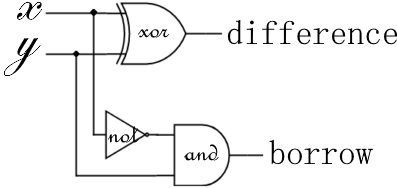
\includegraphics[scale=0.75]{halfsub}
\captionsetup{labelformat=empty}
\caption{Figure 1: The half-subtractor circuit diagram}
\end{figure}
\end{document}